\documentclass[10pt]{article}
\usepackage{multicol}
\usepackage{times}
\usepackage{graphicx}
\usepackage{mathtools}

\addtolength{\oddsidemargin}{-.875in}
\addtolength{\evensidemargin}{-.875in}
\addtolength{\textwidth}{1.75in}

\addtolength{\topmargin}{-.875in}
\addtolength{\textheight}{1.75in}


\begin{document}
\nocite{Gz:5}
\nocite{Gz:6}
\nocite{Gz:7}
\nocite{Gz:8}
\nocite{Gz:9}
\nocite{Gz:10}
\nocite{Gz:11}
\nocite{Gz:12}
\title{A Revised Implementation of the GRAPH/Z Graph Processing System}

\author{
  Ballmer, Alexander\\
  \texttt{alexandersballmer@gmail.com}
  \and
  Moudgalya, Shreyas\\
  \texttt{smoudgal@hawk.iit.edu}
}

\maketitle

\begin{abstract}
  The emerging applications in big data science and social networks has led to the development of several graph-parallel abstractions including GRAPH/Z. GRAPH/Z is a distributed parallel graph processing system running on top of ZHT, a zero hop distributed hash table. It uses an iterative vertex-centric model to store a large graph and run a variety of algorithms over it. GRAPH/Z has some performance issues, and cannot scale the same as Graphlab, a similar commercial framework. We hope to rewrite GRAPH/Z to be competitive with the commercial framework, Graphlab on a single node with multiple threads.  In the previous implementation GRAPH/Z used ZHT, a scalable distributed key-value store as building block. ZHT has very poor data locality, which can create performance issues. We also hope to develop a graph partitioning scheme that can be used in the loading process of GRAPH/Z.
\end{abstract}

\begin{multicols}{2} 
  \section{Background}
  GRAPH/Z was based off of a graph processing paradigm called Pregel. Pregel uses a model centered around the vertexes of the graph.\cite{Gz:1}  Each vertex has an update function that is run in the vertex's context in the graph. Vertexes can modify edges and send messages to other vertexes.\cite{Gz:1} The computation occurs in parallel iterations called supersteps.\cite{Gz:1} At each iteration, vertexes run an update function that can alter the edges around them, or send a message to vertexes in the next iteration. Vertexes can also vote to halt and disable themselves. A halted vertex can be re-enabled by receiving a message. If all the vertexes are disabled at the start of an iteration, the entire system halts and returns.\\
  GRAPH/Z adds a distributed hash table to the Pregel model. The hash table stores the graph, and a distributed message queue that serves as the means of sending messages to the next iteration. The hash table used by GRAPH/Z is ZHT, a DHT implementation that is fault-tolerant and can scale to 32000 cores.\cite{Gz:2}\\
  Graph partition problems are very common to run on systems like GRAPH/Z. Partitioning on graphs falls under the category of NP-hard problems. Solutions to these problems are generally derived using heuristics and approximation algorithms. However, uniform graph partitioning or a balanced graph partition problem can be shown to be NP-complete to approximate within any finite factor. Even for special graph classes such as trees and grids, no reasonable approximation algorithms exist, unless P=NP.\\
  There have been a lot of work to handle big datasets of both commercial and scientific applications, including work flow systems, data streaming management systems and graph databases. These systems typically save the data in distributed file systems(such as Hadoop HDFS and FusionFS), SQL databases(such as Oracle and DB2), and NoSQL database(such as Cassandra and ZHT).\\
  Graph related query is tremendously slow on the traditional relational database, which makes it even more challenging to fully reveal and utilize the scientific and commercial value from the continuously increasing graph data sets. An ideal solution for this problem is to replace the traditional data infrastructure with a graph-centric model, including storage and computing, thus to better serve graph-based applications in terms of performance and programmability.\\
  However, since natural graphs are difficult to partition, the original GRAPH/Z system used ZHT’s hash function to physically distribute all the vertices. As a result, vertices and edges, which are the basic elements of graphs, are spread around different nodes. Due to the random partitioning scheme, when each vertex needs to get access to its edge list, it will statistically communicate to another node and make the communication cost become tremendously higher. Therefore, using hash function to partition the graph data can be considered as a worst case, which is determined by the characteristic of graph structure and the hash function. The original use case of hashing partition is dispersing the data to avoid hot spot, but it doesn’t help in the case of graph processing system.
  
  \section{Problem}
  GRAPH/Z has experienced problems in terms of scaling competitively with commercial software like Graphlab because of the way that ZHT deals with data locality between nodes. ZHT's hashing function does not exploit data locality on one node.\cite{Gz:3} This can cause high network usage and slowdown.\\
  We will also design and implementation a partitioning scheme that works well on the large graph datasets on Graph/Z. The design and implementation of the algorithm must include a fast, balanced and lightweight graph partition scheme based on graph traversal.
  \section{Related Work}
  The closes related system to GRAPH/Z is Pregel. In most of our work, however, we compare GRAPH/Z to Graphlab, which is another high performance graph processing framework. Graphlab uses a similar paradigm to GRAPH/Z, but allows a vertex to access data that is not in a message to the vertex.\cite{Gz:4} \\
  Another less similar but still relevant work is Hadoop, which follows the MapReduce paradigm. GRAPH/Z and Pregel computations can be expressed as a series of chained MapReduce functions.\cite{Gz:4}\\
  Various graph partitioning algorithms exist. Since graph partitioning is a NP-hard problem, practical solutions are based on heuristics. There are two broad categories of methods used. They are local and global. Well known local methods are the Kernighan–Lin algorithm, and Fiduccia-Mattheyses algorithms, which were the first effective 2-way cuts by local search strategies. Their major drawback is the arbitrary initial partitioning of the vertex set, which can affect the final solution quality. Other Global approaches rely on properties of the entire graph and do not rely on an arbitrary initial partition. The most common example is spectral partitioning, where a partition is derived from the spectrum of the adjacency matrix.\\
  A multilevel graph partitioning algorithm works by applying one or more stages. Each stage reduces the size of the graph by collapsing vertices and edges, partitions the smaller graph, then maps back and refines this partition of the original graph. A wide variety of partitioning and refinement methods can be applied within the overall multi-level scheme. In many cases, this approach can give both fast execution times and very high quality results. One widely used example of such an approach is METIS, a graph partitioner, and hMETIS, the corresponding partitioner for hypergraphs.
  
  \section{Proposed Solution}
  Our main work to solve our problems of scalability is to backtrack and try to achieve good scaling on a single node. We believe that the problem with GRAPH/Z lies in bad data locality with ZHT. Our main goal is to achieve some level of competitiveness against GraphLab on a single node, eventually expanding to multi-node scaling through ZHT or another distributed datastore. We will measure performance from weak scaling with larger datasets, and profiling tools such as valgrind/callgrind. The main work will also involve the implementation of a graph partitioning algorithm.
  
  \section{Evaluation}
  We will be using profiling tools such as valgrind and callgrind, along with basic runtime measurement, to measure the efficiency and speed of GRAPH/Z in relation to Graphlab. We will be using a modified pagerank algorithm defined as \\
  $\forall t \in P : r^{(t)}(t)  = (1-\alpha) \cdot r(t) + \alpha \sum_{(s,t) \in L} \frac{r^{(t-1)}(s)}{|L(s)|}$\\ 
  and a graph partitioning algorithm defined as:\\
  Given a graph $G = (V,E)$ and a a set of partitions, $P$, an output partition $V = v_0 \cup V_1 \cup V_2 \cup \ldots \cup V_{p-1}$ such that
  \begin{enumerate}
  \item ${V_i}$ are disjoint $\Rightarrow V_i \cap V_i = \emptyset$
  \item ${V_i}$ are roughly balanced $\Rightarrow |V_i| ~ |V_i|$
  \item let $E_{cut} \equiv {(u,v) | u \in V_i, v \in V_i, i \neq j}$\\
    Minimize $|E_{cut}|$
  \end{enumerate}
  While profiling at a function call level will help us achieve our goal, the metrics used to determine success will be overall runtime and memory use. Scaling will be determined on multiple cores, and increasing data size, but on a single node.  These metrics will be used for the eventual later goal of scaling to more than one node.\\
  These tests will be run on pagerank and the new partitioning algorithm. Results from load balancing tests with other partitioning algorithms such as the Dynamic Cut-Cluster Algorithm, EvoPartition Algorithm, and the Kernighan–Lin Algorithm will be used for comparison. We would also profile the running time of the algorithms based on increase in graph vertices and increase in graph edges.
\end{multicols}

  \section{Timeline}
  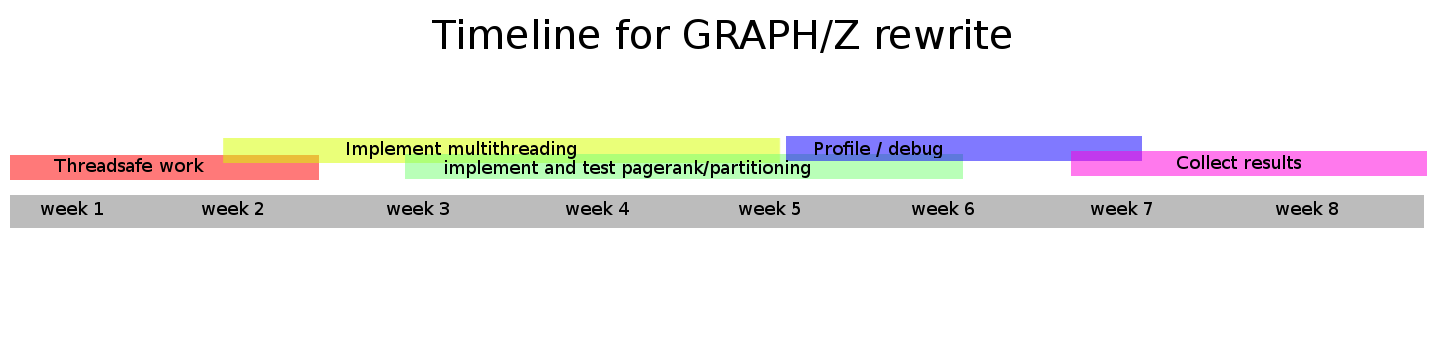
\includegraphics[width=\textwidth]{timeline.png}
\begin{multicols}{2}
  \section{Deliverables}
  We will produce a poster outlining the new GRAPH/Z's strengths and weaknesses and highlighting the changes that we made from the original project. The poster will also include the abstract and writeup needed for entering it into the Supercomputing conference.  Deliverables will also include the finished GRAPH/Z processing system and information comparing it to GraphLab and other existing similar tools. Included on the poster will be data from profiling and traces of the pagerank algorithm and the newly proposed partitioning algorithm on a single node on an instance of AWS EC2 using the dataset from Stanford Network Analysis Project.
  
   \section{Conclusion}
   The original GRAPH/Z was underperforming compared to most other productions graph processing systems. We hope that rewriting it from scratch for a single node will help us pinpoint the cause of the lack of performance. In order to determine if the ZHT distributed hash table is an IO bottleneck, we will confine our implementation to a single node, and use an alternate backend besides ZHT. By using the newly proposed partitioning and pagerank algorithm on GRAPH/Z, we hope to measure better performance of the GRAPH/Z system.
   \bibliographystyle{plain}
   \bibliography{cite}
\end{multicols}
\end{document}
